\section{Analysis}
\label{sec:appendix_analysis}


\begin{figure}[H]
    \centering
    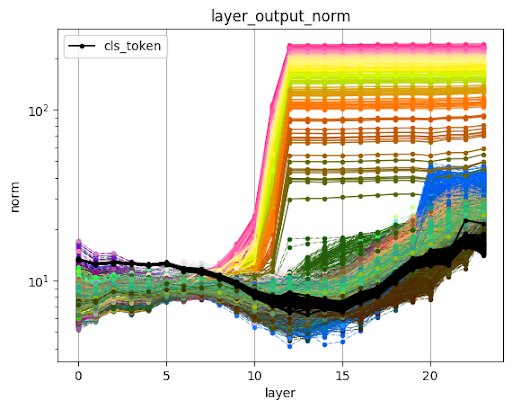
\includegraphics[width=1\linewidth]{figs/massive_token_evolution.png}
    \vspace{-1em}
    \caption{Plot of activation norms of tokens across 50 images over all layers of CLIP ViT-L14 show that the massive tokens become large primarily in layers 11 and 12.}
    \label{fig:massive_token_evolution}
\end{figure}

\subsection{Definitions}
\label{sec:definitions}
Similar to Section \ref{sec:performance_efficiency}, the layer indices used in this section refer specifically to CLIP ViT L-14; however, the same qualitative patterns arise in other large pretrained ViTs. We define two key operations that we will use to analyze the formation of massive tokens:
\begin{definition}[Masking]
    For a vector $w \in \R^n$ and mask $m \in \cb{0, 1}^n$, we define $\sfm$ as \begin{align}
        \sfm(w, m) = \sf(w - \infty \cdot (1 - m)).
    \end{align} In other words, \begin{align}
        \sfm(w, m)_i = \begin{cases}
            \frac{e^{w_i}}{\dss{m_j = 1}{} e^{w_j}}   & \text{if} \ m_i = 1  \\
            0   & \text{otherwise}
        \end{cases}.
    \end{align}
\end{definition}

\begin{definition}[Sinking]
    For a matrix $w \in \R^n$ and mask $m \in \cb{0, 1}^n$, we define $\sfs$ as \begin{align}
        \sfm(w, m) = m \odot \sf(w).
    \end{align} In other words, \begin{align}
        \sfs(w, m)_i = \begin{cases}
            \frac{e^{w_i}}{\dss{j}{} e^{w_j}}   & \text{if} \ m_i = 1  \\
            0   & \text{otherwise}
        \end{cases}.
    \end{align}
\end{definition}

For operand tensors of multiple dimensions, these operations similarly to $\sf$ will only be relevant on the last dimension, while any precedent dimensions will be interpreted as batch dimensions. As a result, we introduce the notations $\attnm{\ell}(\cdot, M)$ and $\attns{\ell}(\cdot, M)$ for the application of Equation \ref{eqn:attn} with the substitution of $\sf(\cdot)$ for $\sfm(\cdot, M)$ and $ \sfs(\cdot, M)$ respectively, as well as $\lyrm{\ell}(\cdot, M)$ and $\lyrs{\ell}(\cdot, M)$ to similarly substitute Equation \ref{eqn:layer}. \\

While masking is common operation frequently used to enable causal masking, pad of heterogeneous sequences, and regularize training, the effect of masking on when applied to a pretrained model is not intuitively clear due to the global rescaling of the attention vector. I.e. for value vector $v \in \R^n$, \begin{align}
    \tr{\sfm(w, m)}v
    & = \frac{\dss{j}{} e^{w_j}}{\dss{m_j = 1}{} e^{w_j}} \tr{(m \odot \sf(w))}v   \\
    & = \frac{\dss{j}{} e^{w_j}}{\dss{m_j = 1}{} e^{w_j}} \dss{m_i = 1}{} \sf(w)_iv_i    \\
    & = \frac{\dss{j}{} e^{w_j}}{\dss{m_j = 1}{} e^{w_j}} (\tr{\sf(w)}v - \dss{m_i = 0}{} \sf(w)_iv_i).
\end{align} Due to the change in the exponential sum, the rescaling of the attention vector may not impact the computational path in a small way, especially if attention weight to a masked token is large which we will observe later. Thus, we identify sinking as a useful intermediate that allows us to study in specific the effects of the additive signal transmitted to a token as a result of the attention mechanism, as we have \begin{align}
    \tr{\sfs(w, m)}v
    & = \tr{\sf(w)}v - \dss{m_i = 0}{} \sf(w)_iv_i.
\end{align}

We identify two masking patterns that will be useful in our analysis of massive token activations, where the patterns regard a set of interest tokens $\mc{T} \subseteq [n]$ with $\mc{T}$ being generally small. \begin{itemize}
    \item We define the \textbf{Type I} masking pattern $M_I(\mc{T})$ as $M$ where $m_{i, j} = \indic{j \notin \mc{T}}$. This means that no token will attend to any token in $\mc{T}$.

    % \item We define the \textbf{Type II} masking pattern $M_{II}(\mc{T})$ as $M$ where $m_{i, j} = \indic{i \in \mc{T} \lor j \notin \mc{T}}$. This means that only tokens in $\mc{T}$ can attend to tokens in $\mc{T}$.

    \item We define the \textbf{Type II} masking pattern $M_{II}(\mc{T})$ as $M$ where $m_{i, j} = \indic{i = j \lor j \notin \mc{T}}$. This means that for all tokens $t \in \mc{T}$, only $t$ can attend to $t$.
\end{itemize}
% These masking patterns are depicted in Figure \ref{fig:masking_patterns}. We refer to the replacement of the $\sf(W)$ operation with $\sfs(W, M_I(\mc{T}))$ as ``\textbf{Type I} sinking set $\mc{T}$'' with identical colloquialism enjoyed for \textbf{Types II} and \textbf{III}. Furthermore, The particular interest sets that we will be applying the masking patterns to will be made explicit in \ref{sec:mechanisms}.
These masking patterns are depicted in Figure \ref{fig:masking_patterns}. We refer to the replacement of the $\sf(W)$ operation with $\sfs(W, M_I(\mc{T}))$ as ``\textbf{Type I} sinking set $\mc{T}$'' with identical colloquialism enjoyed for \textbf{Type II}. Furthermore, the particular interest sets that we will be applying the masking patterns to will be made explicit in Section \ref{sec:mechanisms}.

\begin{figure}[t]
    \centering
    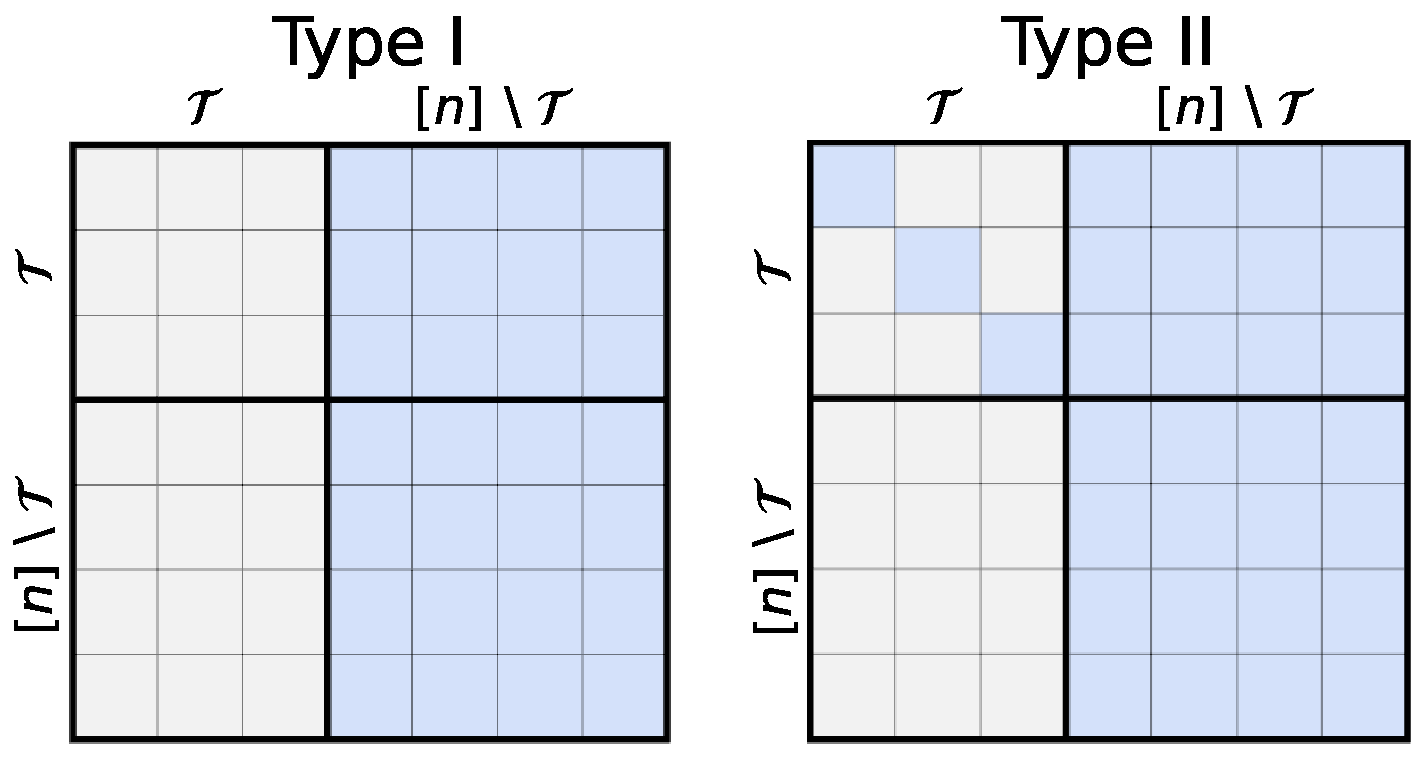
\includegraphics[width=1\linewidth]{figs/masking_patterns_new.pdf}
    \caption{Different masking patterns with respect to the interest set of tokens $\mc{T}$ where blue represents token query-key pairs that are allowed while gray represents query-key pairs that are disallowed.}
    \label{fig:masking_patterns}
\end{figure}


\begin{figure*}[t]
    \centering
    \begin{subfigure}[t]{0.49\linewidth}
        \centering
        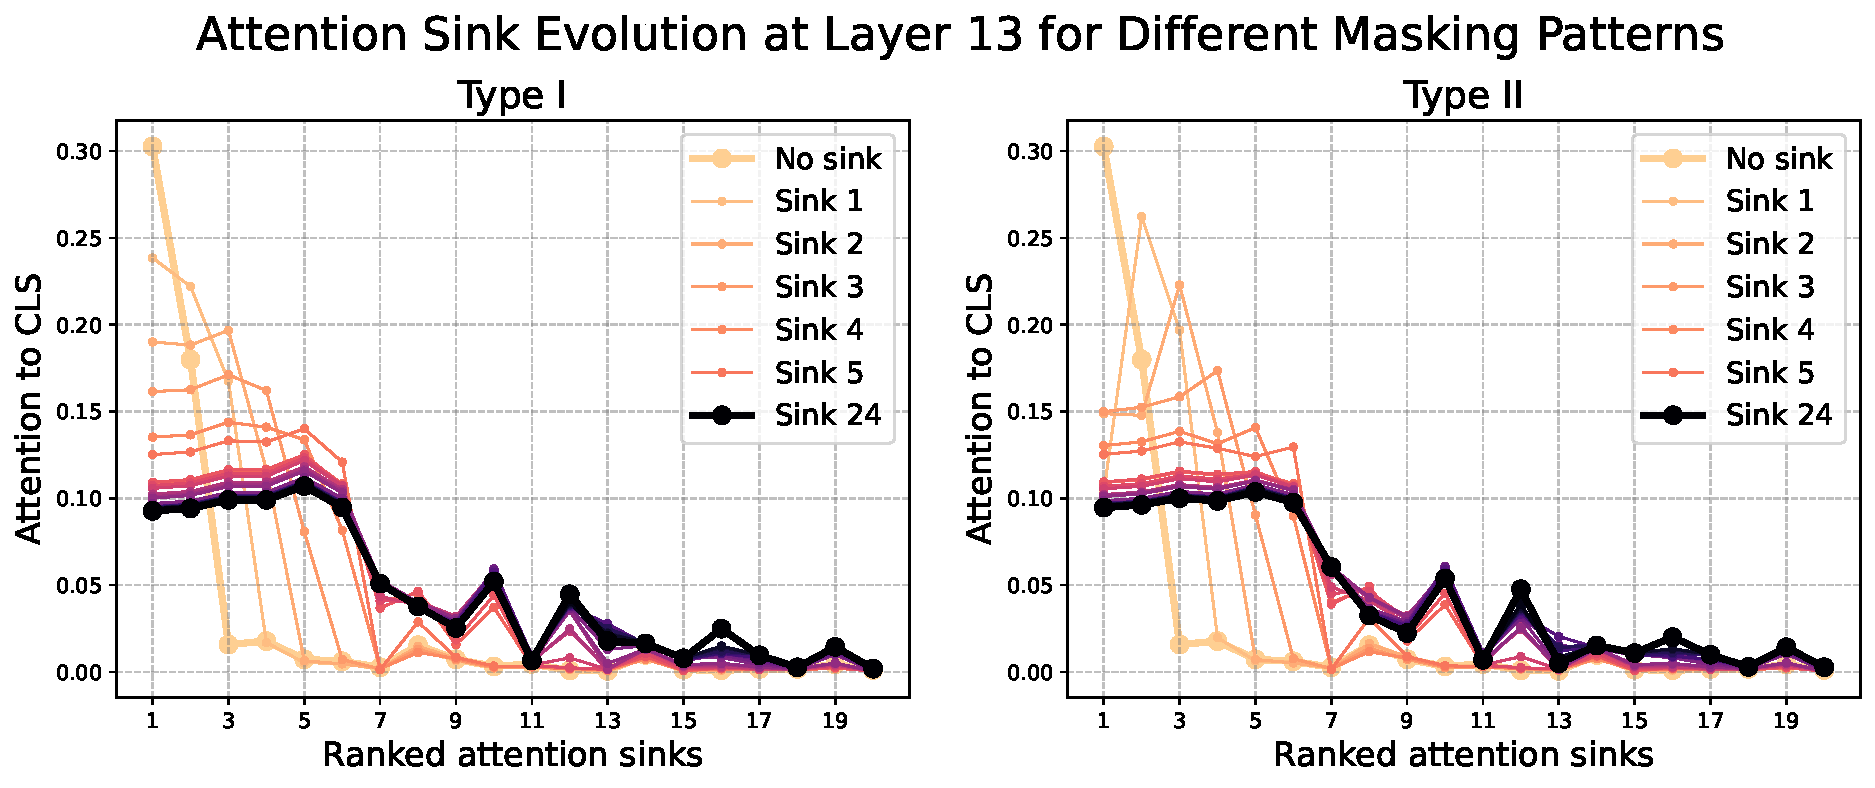
\includegraphics[width=\linewidth]{figs/attention_sink_decay_condensed.pdf}
        \caption{}
        \label{fig:attention_sink_decay}
    \end{subfigure} %
    % \vspace{1em} % Adjust spacing between subfigures as needed
    \begin{subfigure}[t]{0.49\linewidth}
        \centering
        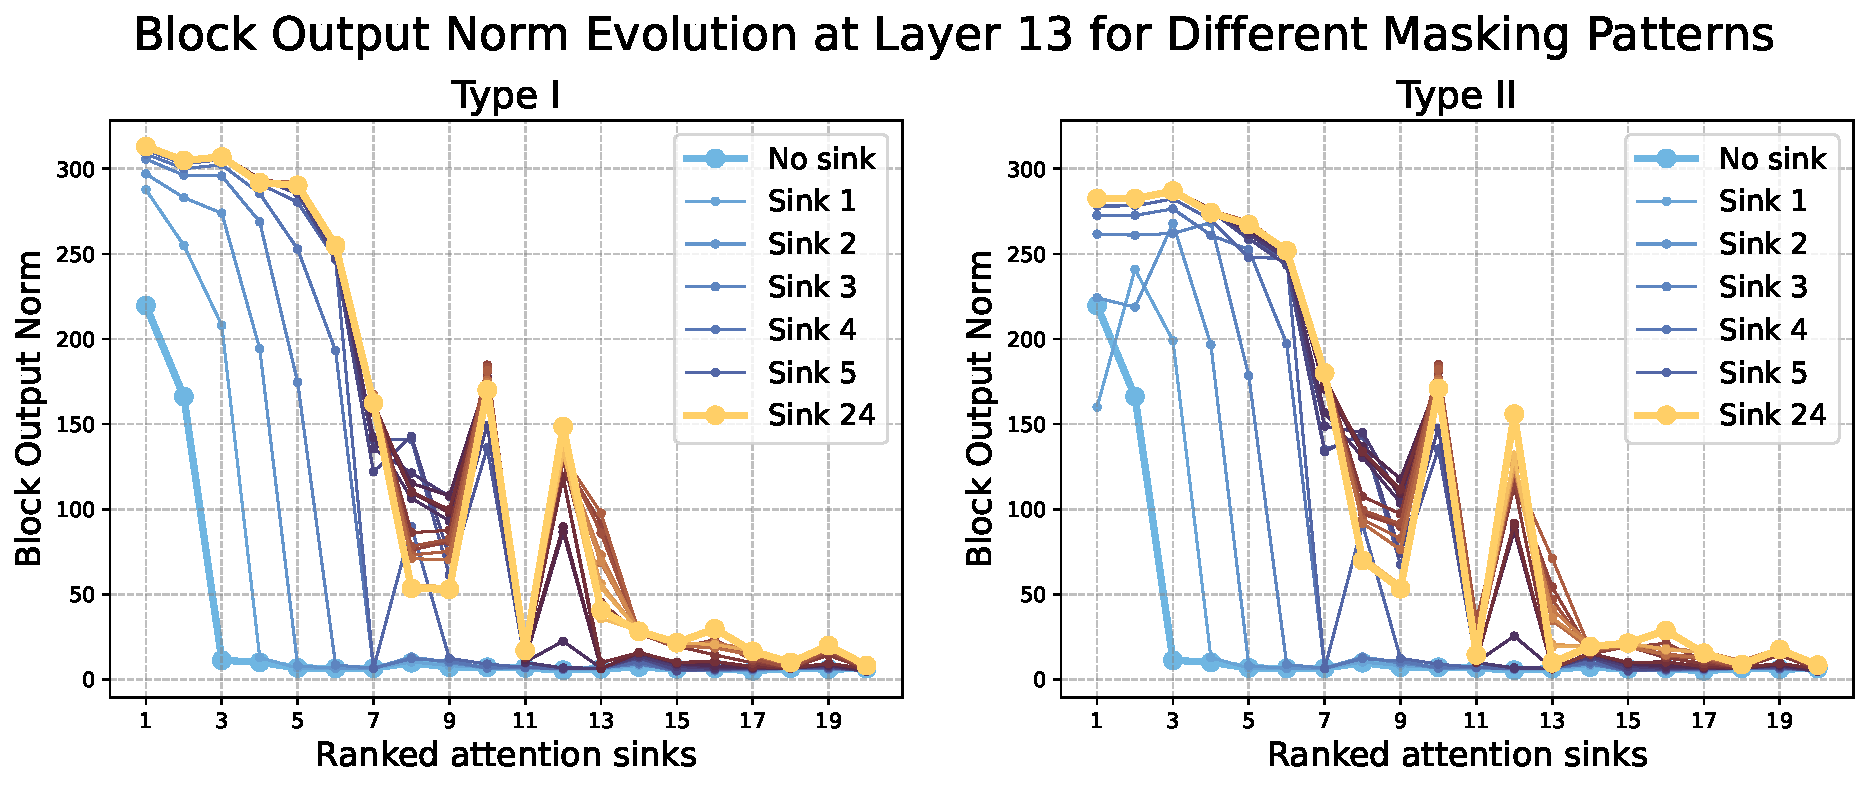
\includegraphics[width=\linewidth]{figs/layer_output_decay_condensed.pdf}
        \caption{}
        \label{fig:layer_output_decay}
    \end{subfigure}
    \caption{The $x$-axis shows individual tokens that are ranked by order of removal in the iterative masking procedure, with the same sequence of top 20 tokens showed for all subplots. The $y$-axis of subfigure \ref{fig:attention_sink_decay} denotes the (unsunk) attention from the CLS token which we use as a more distinct proxy for incoming attention, while the $y$-axis of subfigure \ref{fig:layer_output_decay} denotes the block output magnitude which we determine to be strongly representative of the attention logits. While masking formally redistributes the attention pool across the remaining tokens, sinking can alternatively be interpreted as a zero-ing of values while maintaining the attention weights. Therefore, we observe that iterative masking results in the masked tokens attracting zero attention while subsequent sink tokens rise uncontested. On the other hand, iterative sinking allows sunk tokens the opportunity to ``retain their place'' in the attention distribution which we observe to be diminished but still significant.}
    \label{fig:combined}
\end{figure*}


\subsection{Facilitation of Largeness}
By running the transformer model without the attention mechanism in layers 9 to 12 (through either forwarding the block output $\Emb{\ell}$ direction to $\lyn{2}{\ell}$, or zeroing all attention values i.e. $\sfs(\Wl{\ell}, \mathbf{0})$), we identify the MLP in layers 11 and 12 as the main facilitators of largeness in massive tokens. However, we also observe that \begin{enumerate}[label=\arabic*)]
    \item removing the attention mechanism in layers 9, 10, 11, 12 result in some artifact tokens becoming massive that are not massive in the unmodified computational path, and

    \item for any interest set $\mc{T}$ (including $\emptyset$) that \textbf{Type I} masking or sinking in layers 9, 10, 11, 12 elicits the same set of massive tokens as \textbf{Type I} masking or sinking in layers 9, 10 and proceeding without attention in layers 11 and 12.
\end{enumerate} This suggests that while the MLP in layers 11 and 12 are the main driving force behind making tokens large, the attention mechanism in layers 9 and 10 determines which tokens become massive from a set of potential tokens that is determined by computation up to layer 8.

\begin{figure}[H]
    \centering
    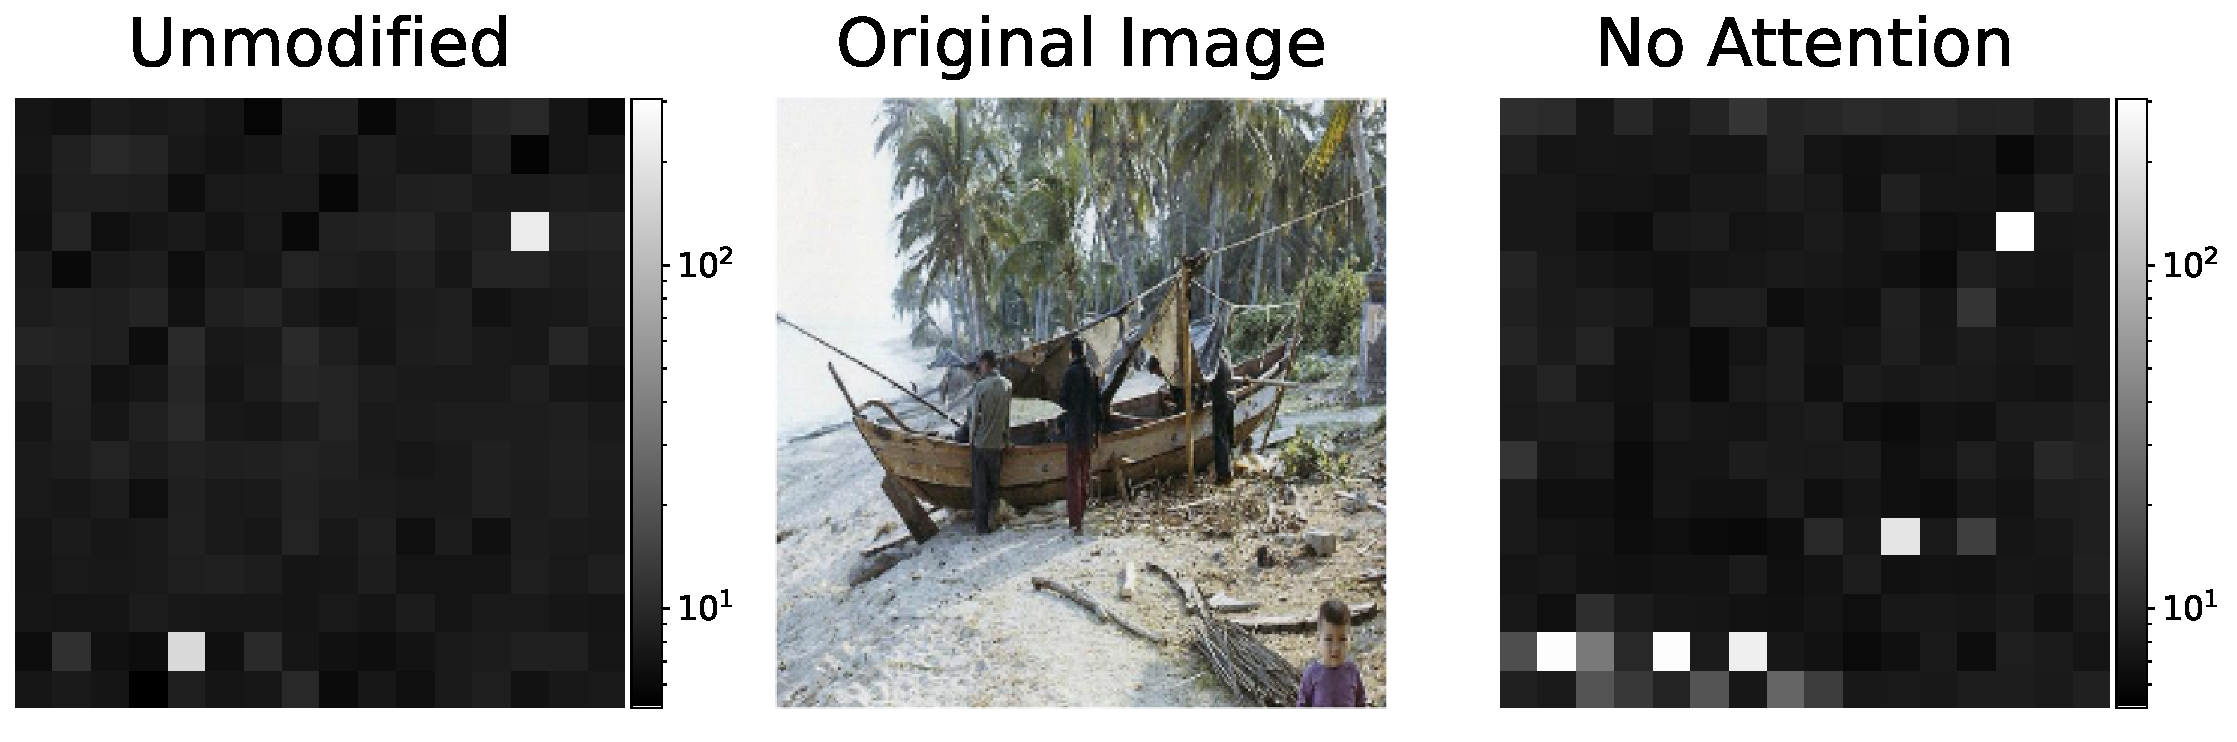
\includegraphics[width=1\linewidth]{figs/mlp_growth_comparison.pdf}
    \caption{Running the model while ignoring the attention mechanism in layers 9, 10, 11, 12 result in some artifact tokens emerging as massive tokens that are not massive in the unmodified computational path.}
    \label{fig:mlp_growth}
\end{figure}

 

\subsection{Intra-Sink Signal Suppression}
\label{sec:suppression}


\subsubsection{Analysis of Type I Masking and Sinking}
We observed in Section \ref{sec:iterative_masking} that iterative masking of attention sinks results in substitute tokens becoming massive as well. However, the same can be said if we instead use iterative \textit{sinking}. However, the difference in results is that even when sinking, the sunk tokens retain their status as attention sinks, albeit diminished. We can see in Figure \ref{fig:attention_sink_decay} that iterative sinking of \textbf{Type I} results in gradual redistribution of attention while the sunk tokens still individually constitute notable fractions of incoming attention. However, we can also observe in Figure \ref{fig:layer_output_decay} that \textbf{Type I} sinking unilaterally increases the size of tokens for multiple iterations. This suggests that in a vacuum, each of the potential sink tokens emit a signal that negatively impacts the ability of other tokens to become large. Removing that signal via masking or sinking allows those tokens to grow. That the incoming attention to the newly sunk token decreases is a result of the saturation of lower-ranked tokens at large magnitudes that are ultimately bounded by Lipschitzness of the MLP.


\subsubsection{Comparison of Type I and Type II Sinking}
With the largest massive token denoted as $t_1$, we then consider what happens when we \textbf{Type II} sink $\cbn{t_1}$ at layers 9 and 10. Because the attention pattern of $t_1$ itself is untouched by \textbf{Type II} sinking $t_1$ alone, its value at the intermediate output of layer 9 is identical to that of unmodified computation. On the other hand, the attention pattern for any token $t \neq t_1$ is identical to that of \textbf{Type I} sinking. Because the MLP applies to individual tokens, we can say in short that the layer 9 output as a result of \textbf{Type II} sinking is unmodified for $t = t_1$, and equivalent to its counterpart in \textbf{Type I} for $t \neq t_1$ as well as larger than its counterpart in the unmodified path.

However, we observe that by the output of layer 10, token $t_1$ under \textbf{Type II} sinking is \textit{smaller} than its unmodified counterpart. Because its value has not changed as of the layer 9 output, this must result from attending to the secondary tokens that have become larger in sinking $t_1$ which immediately suggests that the largeness of the secondary tokens also comes with strengthened suppression signals. This reversal effect compounds up until layer 13 by which token $t_1$ is significantly smaller than its unmodified counterpart as seen in Figure \ref{fig:layer_output_decay}.

% Finally, we observe that the \textbf{Type II} sinking pattern under many iterations converges to the identity mask in which each token is effectively only suppressing itself. Alternatively, every potential sink token at the limit receives the benefit of no longer being suppressed by other tokens, which is of greater significance for lower ranked tokens. Therefore, we observe the same limiting redistribution behavior for \textbf{Type II} as for \textbf{Type I}, while also observing early plummets in incoming attention and activation norm at the early stages of iterative removal.





